% ============================================================
% Pinning the Wage to Scarcity and Technology
% Generated from paper/pinning.html by code/html_to_latex.py.
% The HTML stays canonical: edit there, re-run the converter.
% ============================================================
% Style: orthodox macro working paper (12pt, onehalf spacing, plain theorem
% style with italic statements, numbered equations, CM fonts).
\documentclass[12pt]{article}
\usepackage[T1]{fontenc}
\usepackage[utf8]{inputenc}
\usepackage[a4paper, margin=2.5cm]{geometry}
\usepackage{setspace}
\onehalfspacing
\usepackage{amsmath, amssymb, amsthm}
\usepackage{bm}
\usepackage{graphicx}
\usepackage{booktabs}
\usepackage[labelfont=bf, labelsep=period, font={footnotesize,stretch=1}, justification=justified]{caption}
\usepackage{microtype}
\usepackage{titlesec}
\usepackage[hidelinks]{hyperref}

\theoremstyle{plain}
\newtheorem{proposition}{Proposition}
\newtheorem{lemma}[proposition]{Lemma}
\newtheorem*{corollary}{Corollary}

% hanging-indent entry for the hand-formatted reference list
\newcommand{\refentry}[1]{\par\hangindent=1.5em\hangafter=1\noindent #1}

\title{\bfseries Pinning the Wage to Scarcity and Technology\thanks{Views are the
  authors' own and do not represent those of KTH, SEB, or the Stockholm School of
  Economics. Written in collaboration with Claude (Anthropic); see the AI-use note
  at the end.
  % NOTE (generated): the HTML draftline reads "Views are the author's own and do
  % not represent those of KTH or SEB." — pluralized and extended to SSE when the
  % co-author was added. Reword as needed.
  }\\[7pt]
  \large\mdseries Replacement, exit, and the rents of non-produced inputs in a task economy}

% Author order: Wilson first (her call, 2026-08-21).
\author{Stella Wilson\thanks{KTH Royal Institute of Technology and Skandinaviska
    Enskilda Banken (SEB). Email: \texttt{thmwi@kth.se}.}
  \and
  Johan B\r{a}ge\thanks{Stockholm School of Economics.
    Email: \texttt{Johan.Bage@hhs.se}.
  }}

\date{Working draft --- August 2026}

\begin{document}
\maketitle

\begin{abstract}
\noindent In a task model the wage is priced against its machine substitute, which is the cost of the machine adjusted by the difference in productivity at equilibrium, $w = c\cdot \gamma (x^*)$. We price that substitute on its own production: free entry gives that it depends on replacement costs, human labor costs and cost of raw materials. $c = ac + \lambda w + br$. Thus as machine production sheds labor, replacement cost resolves into rents on non-produced inputs --- land, sites, energy. Margin and recursion together pin the wage to scarcity and technology: $w = \gamma (x^*)\cdot br/(1 - a - \lambda \gamma (x^*))$. We price market exit from the same inputs: leaving the labor market still requires housing, space, and energy, so the same rents lower the outside option. At uniform machine capability, real wages diverge by what they are measured in: in machine-made goods the wage is pinned by absolute human productivity; against housing, space, and energy it falls without bound. In the U.S. since 1964 these two measures now diverge with a factor of 4.8: the same average paycheck buys nearly four times the durables or a fifth less shelter. From the model we derive a taxation and benefit system: a tax on the rents of non-produced inputs funding a uniform per-person transfer. It distorts no production decision and changes no work--exit choice. We find that taxed in full, U.S. site rents would fund one-third of a per-person subsistence floor today, up from a twentieth in the 1950s.
\end{abstract}
% TODO: JEL codes and keywords for the title page — suggestions,
% to be confirmed by the authors:
% \noindent JEL: E25, J23, O33, H21. \quad
% Keywords: automation, tasks, wages, land rents, outside option.

\section{Introduction}\label{sec:intro}

Suppose a firm can perform a task with a worker or with a machine. For the tasks where the firm is indifferent, the worker's wage is tied to the cost of the machine substitute. That mechanism is established and used by the factor-price condition at the task margin in Acemoglu and Restrepo (2018), with the same threshold logic in Zeira (1998) and, for tasks that move abroad rather than to machines, in Grossman and Rossi-Hansberg (2008). This paper examines that mechanism with two questions around that margin.

\textbf{What prices the substitute?} A machine is itself produced --- from other machines, labor, energy, sites, minerals, permissions. Its rental is an equilibrium object. Follow that price backward through production and it terminates in inputs whose supply does not expand with production itself: land is the permanent example; a grid connection, a mineral right, or a fabrication bottleneck can hold the same position over shorter horizons. While machine production still employs labor, part of the machine's cost will be the wage itself, and thus the substitute will remain relatively expensive. As machine production sheds labor, that cost component is reduced, and the replacement price resolves increasingly into terminal rents.

\textbf{What prices the alternative to working at all?} A worker sells an hour when the wage beats the best alternative use of that hour. Life outside the market wage still requires somewhere to live, food, energy, warmth, and usually access to a household. The value of exit is therefore also a price --- and it depends on the same scarce inputs that anchor the machine's cost. When machine-made goods cheapen while housing and energy do not, the exit option deteriorates in exactly the units that matter to the person weighing it.

This paper closes both prices around the labor margin:
\[
\textit{wage supply} \to \textit{machine substitute} \to \textit{the machine's inputs} \to \textit{rents on non-produced inputs}
\]
on the labor demand side, and
\[
\textit{wage demand} \to \textit{exit} \to \textit{the inputs of unwaged life} \to \textit{rents on non-produced inputs}
\]
on the labor supply side. The wage sits in an interval, with replacement cost, the opportunity cost for firms paying wages, above and exit value, the opportunity cost for workers performing tasks, below, and both endpoints of these opportunity costs are formed partly in the market for non-produced inputs. Technological change moves both at once. It changes what workers can do relative to machines at final tasks and it changes how much labor the machine's own production employs. Crucially, it also changes the relative price of the scarce inputs that both chains terminate in.

We can illustrate this dynamic with the extreme scenario. Suppose machine capability becomes uniform across tasks. Thus machines are at rough parity with humans everywhere, and there exists no task where the human competitive advantage is large. In that limit every standing account of the wage becomes degenerate: there is no marginal-product schedule to climb, no bargaining surplus to split, no scarcity of labor for population to price. What remains is a simple set of constraints: the wage in machine-made goods is pinned by absolute human productivity and cannot fall (a point proved by Caselli and Manning (2019)), while the wage against housing, space, and energy falls to near zero as the capability gap closes, because that is where the value released by automation settles. The real wage forks by the composition of goods and labor used in production, a process which is visible in U.S. measurements in Section~\ref{sec:measurement}.

Applying the task margin model of Acemoglu and Restrepo and adding a price recursion mechanism based on the input-output logic of Leontief (1936) and Sraffa (1960) we are able to derive a closure of the wage model. We price the machine rental from its own production recursion and substitute it into the task margin, so the wage is expressed in terminal rents and the transition rides on a measurable parameter, the labor content of machine production. We price the outside option in the same relative price, so both endpoints of the bargaining interval move on one variable. From those two closures we derive the fork and its fiscal completion, a re-derivation of George (1879): a rent tax funding a uniform transfer, the pair that continues to function in the limit.

Section~\ref{sec:accounts} surveys how current theory tries to pin the wage. Sections~\ref{sec:model}--\ref{sec:floor} build the model: the margin, the ceiling, the floor. Section~\ref{sec:interval} closes the wage interval. Section~\ref{sec:limit} analyses the limit case and states the fork. Section~\ref{sec:fiscal} states the fiscal completion. Sections~\ref{sec:history}--\ref{sec:measurement} applies the model to modern economic history using U.S. measurements. Section~\ref{sec:stabilizers} weighs the possible stabilizers. Section~\ref{sec:ai} draws the implications for artificial intelligence. Everything supporting but not essential to the model --- the general machine sector, the closed-economy identity, the fiscal system away from the limit, human-essential tasks --- is in the appendix.

\section{What standing accounts pin the wage to}\label{sec:accounts}

Accounts of the aggregate wage differ less in their mechanisms than in where they stop. Each family below determines the wage relative to a quantity that labor itself helps produce, or leaves it inside an interval whose endpoints it takes as given, or determines its growth rate while not fixing its level. We do not offer the model of Sections~\ref{sec:model}--\ref{sec:floor} against them; instead the objects at which they terminate.

\subsection{Marginal product}\label{sec:marginal-product}

The textbook answer sets the wage equal to the marginal product of labor. As a statement about competitive equilibrium it is correct, and this paper's Proposition~\ref{prop:margin} is an instance of it: $w = c\cdot \gamma (x^*)$ (using our notation, see Section~\ref{sec:model}) is the marginal product, evaluated at the margin the machine alternative sets. What the identity does not supply is a level: the marginal product is a function of the capital stock and the technology, two variables constantly changing. Applied work usually proceeds under Cobb--Douglas, which requires fixed factor shares and an aggregate capital measure. This makes it fragile when considering times of rapid changes to the factor shares. Likewise the aggregate capital measure becomes uncertain when the price of capital is the underlying factor analysed (Sraffa 1960; Samuelson 1966). In growth theory the wage's growth rate is pinned along a balanced path, but Uzawa (1961) shows the balanced path requires technical change to be labor-augmenting in form --- and the form of technical change is precisely what is at issue under automation.

\subsection{Search, matching, and bargaining}\label{sec:search}

The search-and-matching framework (Diamond 1982; Mortensen and Pissarides 1994; Pissarides 2000) places the wage between the worker's outside option and the value of the match, dividing the surplus by a bargaining parameter. The framework is explicit that the level is not determined within it: two endpoints and a split, and it supplies none of the three.

Shimer (2005) showed that the calibrated model generates almost none of the observed volatility --- in U.S. data the vacancy--unemployment ratio is roughly twenty times as volatile as labor productivity, while the model makes them comparable. Hagedorn and Manovskii (2008) resolve the puzzle by setting the value of non-market activity close to productivity, so that the surplus workers and firms split is small; Hall (2005) resolves it with rigid wages; and Ljungqvist and Sargent (2017) show that these and the other proposed resolutions operate through one channel, the \emph{fundamental surplus} --- ``an upper bound on the fraction of a job's output that the invisible hand can allocate to vacancy creation'' --- which every successful calibration makes small, and whose leading deduction from productivity is the value of non-work. The central calibration debate of modern macro-labor is, in other words, a debate about the level of an object the framework treats as a parameter.

We supply both endpoints. Section~\ref{sec:ceiling} prices the upper wall (what the firm's machine alternative costs, and why); Section~\ref{sec:floor} prices the lower wall (what the worker's exit is worth, and why); and Section~\ref{sec:interval} observes that the two are formed partly in the same market, so they can move together --- and in the automation limit, close.

\subsection{Task and assignment models}\label{sec:tasks}

The task framework (Zeira 1998; Acemoglu and Autor 2011; Acemoglu and Restrepo 2018, 2022) determines the wage at the threshold task and is the direct ancestor of what follows. Its equilibrating force is the creation of new labor tasks: displacement met by reinstatement (Acemoglu and Restrepo 2018; Autor 2015). In each version the machine rental and the outside option enter as parameters; the wage is passed through the threshold rather than determined at it. This paper closes both parameters, and holds the new-task margin shut. The latter is a modelling assumption we make based on our reading of history and recent U.S. measures. Acemoglu and Restrepo (2026) add institutional wage wedges and show that automation is directed at the tasks where wedges are largest; Section~\ref{sec:stabilizers} states that result in this notation. Cross border trade is treated similarly: a tradable task stays domestically only while the wage beats both the machine rental and the foreign wage, so the foreign wage is a second machine rental with a different cost composition. Offshoring is however still only a temporary condition, once the machine undercuts the foreign worker, the task flips onward to machines wherever they sit.

\subsection{Institutional accounts}\label{sec:institutions}

Efficiency wages (Shapiro and Stiglitz 1984), monopsony (Manning 2003), and firm-level rent sharing (Card, Cardoso, Heining, and Kline 2018) explain why individual wages depart from a common base and why the dispersion moves. In the notation below they are accounts of a multiplicative wedge on particular tasks. The model takes them as given at that layer and focuses instead on the common base.

\subsection{The classical accounts}\label{sec:classical}

The wage was pinned to land and to the cost of subsistence before it was pinned to anything else. Ricardo (1817) priced land at the margin and the wage at its natural price, Malthus (1798) supplying the mechanism; the machinery chapter added in 1821 concedes that machinery can injure the laboring class. Marx priced labor power at its cost of reproduction and read enclosure --- the legal extinction of common access to land --- as the manufacture of a labor supply. Lewis (1954) pinned the modern-sector wage to what the traditional sector affords --- the closest antecedent to Section~\ref{sec:floor}, differing in that his traditional sector is exhausted by absorption rather than priced away by rent. Polanyi (1944) recorded the institutional half of the same event. George (1879) drew the fiscal consequence this paper's Section~\ref{sec:fiscal} derives inside the model. These accounts were not refuted. The premise they shared --- that the human advantage over tools varied little from task to task --- stopped holding, and the conclusions lapsed with it. Section~\ref{sec:history} reads the classical case as the flat configuration of the schedule built below.

\subsection{Automation and the wage}\label{sec:automation}

Korinek and Stiglitz (2019) pose the below-subsistence scenario this model resolves through exit; Korinek and Suh (2024) is the closest formal predecessor on wage collapse under transformative AI, differing in where the collapse ends --- here at non-produced factors rather than accumulated capital --- and in the treatment of the outside option. Susskind (2017) and Sachs and Kotlikoff (2012) reach technological immiseration through other channels; Moll, Rachel, and Restrepo (2022) route automation's gains to wealth-holders, where this model names the terminal claimant. Aghion, Jones, and Jones (2019) supply the strongest stabilizer --- expenditure concentrating on whatever remains human-essential --- granted a theorem in Appendix~\ref{app:human}. Caselli and Manning (2019) prove real wages cannot fall in terms of machine-made goods; Section~\ref{sec:limit} concedes the theorem and locates the fall elsewhere. Hémous and Olsen (2022) endogenize automation's direction.

\subsection{Where the model meets data}\label{sec:data}

Three empirical literatures serve below as instruments. Factor shares: the labor share's decline is documented and global (Karabarbounis and Neiman 2014), and its capital-side counterpart resolves substantially into housing --- which is to say land (Rognlie 2015; Knoll, Schularick, and Steger 2017; Piketty and Zucman 2014). The long wage record: real wages measured against the cost of a subsistence basket --- welfare ratios in the sense of Allen (2001), extended for England by Clark (2005) --- are the same object this paper refers to as the floor, computed at the household level; Section~\ref{sec:history} describes that record. Payroll incidence: under Proposition~\ref{prop:margin} the share of a payroll tax borne by workers maps to the inverse slope of the schedule at the margin, so the quasi-experimental incidence literature (Gruber 1997; Kugler and Kugler 2009; Saez, Schoefer, and Seim 2019) is, in this model, a repeated measurement of the schedule's flattening; Section~\ref{sec:measurement} specifies that assembly --- existing estimates compiled onto one pass-through definition --- as open work.

\section{The model: tasks and the margin}\label{sec:model}

\textbf{Tasks.} Producing one unit of the final good requires a continuum of tasks $x \in$ [0,1], each in equal amount (Leontief aggregation over tasks): the good's unit cost is the sum of its tasks' unit costs. One human-hour completes $\gamma _L(x)$ units of task $x$; one machine-hour completes $\gamma _M(x)$. Relative human productivity is
\begin{equation}\label{eq:gamma}
\gamma (x) = \gamma _L(x) / \gamma _M(x).
\end{equation}

A machine-hour rents for $c$ --- a parameter here, the subject of Section~\ref{sec:ceiling}. Institutional wage wedges --- union premia, licensing rents, efficiency wages --- are set aside until Section~\ref{sec:stabilizers}.

\textbf{People and land.} $N$ identical workers each supply one hour or exit to an outside option worth $s$ --- the value of the best life available without selling labor. $s$ is a parameter here and the subject of Section~\ref{sec:floor}; it presupposes somewhere to live. Land is fixed in total, heterogeneous in quality, with the worst parcel's reservation rent zero.

Labor, at wage $w$, holds task $x$ when it is the cheaper input: $w/\gamma _L(x) \le c/\gamma _M(x)$, i.e. $w \le c\cdot \gamma (x)$. Relabel tasks so $\gamma$ increases, and assume the relabeled schedule is continuous and strictly increasing where labor is employed (flat stretches are handled in Appendix~\ref{app:environment}). Competitive assignment then produces a threshold $x^*$: machines take [0, $x^*$), labor takes $[x^*, 1]$ (Figure~\ref{fig:schedule}).

\begin{proposition}[the task margin]\label{prop:margin}
(i) In any equilibrium using both inputs, $w = c\cdot \gamma (x^*)$. (ii) The wage's sensitivity to labor supply is governed by the slope of $\gamma$ at $x^*$: a steep schedule makes labor demand inelastic and the wage unresponsive; as the schedule flattens toward a constant $\bar{\gamma}$, labor demand becomes perfectly elastic at $c\cdot \bar{\gamma}$ and the wage is pinned there regardless of how many or few workers exist. (iii) No equilibrium wage sits below $s$ while anyone works: if the clearing wage would fall below $s$, workers exit until the wage recovers to $s$ (possible only where the schedule has slope) or all have left.
\end{proposition}

\begin{proof}
(i) If $w > c\cdot \gamma (x^*)$, the marginal task and, by continuity, tasks just above it are cheaper by machine; firms drop labor there and the unemployed underbid. If $w < c\cdot \gamma (x^*)$, tasks just below $x^*$ strictly favor labor and bidding raises $w$. Only equality is stable. (ii) Absorbing more hours requires labor to win more tasks, and a firm concedes a task only when the wage falls relative to that task's machine cost; the required fall is proportional to the slope. At a flat schedule no wage above $c\cdot \bar{\gamma}$ employs anyone and every wage at $c\cdot \bar{\gamma}$ employs everyone willing. (iii) is the participation condition applied to (i) and (ii). Existence and uniqueness of $(w, x^*)$ are Lemma~\ref{lem:existence}.
\end{proof}

The condition is an indifference: the worker has no cost advantage at the marginal task; what is being priced is relative productivity. If $c = \$10$ and $\gamma (x^*) = 4$, the marginal worker can be paid \$40 while leaving the firm indifferent. Let machines improve uniformly by 25\%, so $\gamma (x^*)$ falls to 3.2: the same worker's ceiling is \$32 --- a 20\% cut delivered entirely by someone else's machine improving at her task, with no human getting worse at anything. That arithmetic holds $c$ fixed while machines improve, and machine progress also cheapens machine-made goods.

\begin{figure}[t!]
\centering

\includegraphics[width=0.88\linewidth]{figures/fig_schedule.png}
\caption{The task-assignment margin. Tasks are ordered so $\gamma (x)$ increases; the ratio $w/c$ divides them: machines hold every task with $\gamma (x) < w/c$, labor holds every task above, and at $x^*$ the two inputs cost the same. Anything that lifts the line --- a costlier worker or a cheaper machine --- shifts tasks to machines; anything that lowers $\gamma$ near the margin does the same at a fixed line. The two automation channels of Section~\ref{sec:ceiling} are exactly those two movements.}
\label{fig:schedule}
\end{figure}

\section{The ceiling: what prices the machine}\label{sec:ceiling}

Proposition~\ref{prop:margin} prices labor off the machine; this section prices the machine off its recipe. Suppose one unit of machine services is produced with three kinds of inputs: $a$ units of machine services themselves ($a < 1$: machines net-reproduce); $\lambda$ labor-hours --- the fabrication, operation, maintenance, and installation the machine sector still buys; and $b$ units of non-produced services --- sites, energy, ore --- renting at $r$, the rent of the sites production uses (parcels differ in quality; Appendix~\ref{app:landonly} specifies the schedule). As a price equation this is the one-sector version of the input-output cost systems of Leontief (1936) and Sraffa (1960): with free entry and constant returns, the rental equals unit cost,
\begin{equation}\label{eq:recursion}
c = a\cdot c + \lambda \cdot w + b\cdot r.
\end{equation}

The first term is recursively embodied machine content; the second is the wage bill inside the substitute; the third is the claim on the inputs at which the recursion terminates. Call an input \emph{terminal}, informally, when its supply does not expand through the production process itself on the horizon under study; the propositions say ``non-produced.'' Land is the permanent case. Energy capacity, transmission, minerals, and fabrication bottlenecks can occupy the position for years at a time and then leave it as they are completed or resolved; Section~\ref{sec:ceiling}'s results hold over whatever horizon the classification holds, and our long-run claims use the permanent case.

\begin{proposition}[replacement closure]\label{prop:replacement}
Let the task margin hold, $w = c\cdot \gamma ^*$, with $\gamma ^* = \gamma (x^*)$, and let machine services be priced by free entry, $c = ac + \lambda w + br$. If $1 - a - \lambda \gamma ^* > 0$, then
\begin{equation}\label{eq:closure}
c = b\cdot r / (1 - a - \lambda \gamma ^*),\qquad w = \gamma ^*\cdot b\cdot r / (1 - a - \lambda \gamma ^*).
\end{equation}

The wage is a claim on terminal rents, scaled by relative productivity at the margin and amplified by the recursion. On the viable set both prices rise in $\lambda$ and in $\gamma ^*$.
\end{proposition}

\begin{proof}
Substitute $w = c\gamma ^*$ into the zero-profit condition: $c = ac + \lambda c\gamma ^* + br$, so $c\cdot (1 - a - \lambda \gamma ^*) = br$. Multiply by $\gamma ^*$ for the wage. The derivatives are $\partial w/\partial \lambda = \gamma ^{*2}br/(1-a-\lambda \gamma ^*)^2$ and $\partial w/\partial \gamma ^* = br(1-a)/(1-a-\lambda \gamma ^*)^2$, both positive; and $\partial c/\partial \gamma ^* = \lambda br/(1-a-\lambda \gamma ^*)^2$, positive exactly when $\lambda > 0$.
\end{proof}

The viability condition has an intuitive reading: $a + \lambda \gamma ^*$ is the produced content of one unit of machine services once its labor is priced at the margin --- direct machine content $a$, plus the machine-equivalent $\lambda \gamma ^*$ of its labor. If that reaches one, the sector cannot deliver services at any finite price.

The formula separates two kinds of automation that are usually discussed as one.

\textbf{Task automation} lowers $\gamma ^*$: machines improve at tasks near the assignment margin, so a marginal human hour replaces less machine service. This is the automation of the task literature.

\textbf{Recursive automation} lowers $\lambda$: fewer human hours are required to produce, operate, and maintain machine services themselves. This removes the wage bill from the substitute's own cost base and cheapens the substitute directly.

Either change lowers the wage supported by a given terminal rent. And they interact: with $\lambda > 0$, task automation also cheapens the machine, because it cheapens the machine sector's own labor. A worked instance, showing the recursion's amplification: at $(a, \lambda , \gamma ^*, b, r) =$ (0.5, 0.1, 3, 0.2, 1), the recipe gives $c = 1$ and $w = 3$, and one checks 1 = 0.5$\cdot$1 + 0.1$\cdot$3 + 0.2$\cdot$1. Now let recursive automation run $\lambda$ from 0.1 to 0, holding everything else fixed: $c$ falls to 0.4 and the wage falls to 1.2 --- a 60\% cut from removing one tenth of an hour of labor from the machine recipe, because that tenth of an hour, priced at the margin wage, was 30\% of the recipe's cost. In the limit $\lambda \to 0$,
\begin{equation}\label{eq:lambda-zero}
c \to b\cdot r/(1 - a),
\end{equation}
and the replacement price contains no wage at all: its reproducible components are internal to the recursion, and what remains in unit cost is the claim on the terminal input. (Time preference and durability add an interest term to the recursion but do not change the conclusion; Appendix~\ref{app:environment} has the derivation, along with the matrix version for many machine types and several terminal inputs.)

\textbf{Ideas are the boundary case.} An idea's reproduction requires approximately nothing of anything, so its competitive price is approximately zero; any positive price on an idea is institutional scarcity, chosen --- and chosen for a reason Romer (1990) made canonical: at marginal-cost pricing, ideas with fixed creation costs are not created. Institutional rents are therefore real, revocable, and policy-elastic; the taxonomy of Section~\ref{sec:limit}'s corollary keeps a column for them without confusing them with the physical kind.

\section{The floor: what prices exit}\label{sec:floor}

The task margin says what a firm will pay. A worker accepts when the offer beats the value of the best alternative --- the outside option $s$ of search theory, the reservation value of participation models. In most labor models $s$ is a parameter, and for short-run questions that is exactly right. For long-run technological change it conceals a price, and the concealment matters, because the empirical debate of search and matching is changed significantly on this object's level.

Exit is a consumption problem. A person who leaves the labor market lives on household production, family, savings, transfers, informal work, a plot --- and every one of those arrangements uses housing, space, energy, food, and care. Field evidence prices the components: the value of non-work time and household production is substantial and heterogeneous (Mas and Pallais 2019), and the calibration that resolves the volatility puzzle sets the aggregate outside option high for exactly this reason (Hagedorn and Manovskii 2008). If the inputs of unwaged life become expensive relative to goods, the value of exit falls with no change in anyone's capabilities.

Model the exit life directly. Let $q = r/p$ be the price of non-produced services relative to the goods price $p$ (the machine-made good is the numeraire below). An independent exit arrangement yields a keep $s_0$ in goods units and requires $h_e$ units of land services --- quality-adjusted, so no particular parcel is needed. If no plot is affordable, exit degrades to a dependency floor $\underline{s} < s_0$: living on someone else's land, at someone else's sufferance --- in the modern economy, most often a parent's spare room. So
\begin{equation}\label{eq:exit}
s(q) = \max( s_0 - q\cdot h_e , \underline{s} ),
\end{equation}
falling one-for-one with $q\cdot h_e$ until the dependency floor binds; from there, further rent increases find nothing in the exit bundle left to price. The functional form is deliberately minimal; the only essential property is $\partial s/\partial q \le 0$, and the caveat is that an exit provisioned with machine-made goods adds a falling goods term --- the conclusion stands wherever the exit bundle keeps a positive non-produced share, which is the same condition within the fork of Section~\ref{sec:limit}.

\begin{proposition}[priced exit]\label{prop:exit}
(i) While suitable parcels lie idle --- parcels on which the keep $s_0$ is attainable --- the marginal such parcel rents at zero: the exit plot is free and $s = s_0$. An unpriced margin of this kind is what ``a commons'' is, economically: idle land, family access, public provision --- any arrangement supplying the scarce input below its scarcity rent. (ii) Once no suitable parcel lies idle, the exit plot pays the ruling rent and $s = s(q)$ above. The trigger is land scarcity, not machine capability: the mechanism operates in the sloped regime ($\gamma$ still sloped at the margin), where the evidence lives. (iii) For workers with $\partial s/\partial q < 0$, a rise in $q$ shifts labor supply outward: participation weakly rises, and by Proposition~\ref{prop:margin}(ii) the equilibrium wage weakly falls where the schedule has slope (at a flat schedule the wage is pinned and only participation moves).
\end{proposition}

\begin{proof}
(i) Any positive rent on the marginal parcel is undercut by an idle neighbor of reservation rent zero. (ii) With no idle neighbor, the exit plot must outbid other uses for the marginal suitable parcel, whose rent is now positive; the keep is $s_0 - q\cdot h_e$ until $\underline{s}$ binds. (iii) A lower reservation value moves the participation step down: more workers accept at any wage; the wage response is Proposition~\ref{prop:margin}'s comparative statics.
\end{proof}

A parcel rents at zero because little can be done with it --- which is why the truly idle margin supports no exit either. Free and livable together is a particular historical configuration: the commons proper, and its closing is the enclosure read below. When no suitable parcel idles, the floor $\underline{s}$ is not land-free but otherwise-funded, in three modern forms: dependency --- a room supplied out of someone else's wage or ownership, an unpaid transfer from the employed to the exited; public provision --- the out-of-work payment of Appendix~\ref{app:conditionality}, unconditional in few places and thin where it exists; and tolerated use --- living on land one does not hold, its price paid in eviction risk rather than rent. Each is a commons in the degraded sense: the scarce input supplied below its rent, from someone's budget, the state's, or the law's forbearance. None is insulated from $q$: the host's capacity to share inherits the host's rent bill, so the flat segment at $\underline{s}$ is an upper bound, and Appendix~\ref{app:race}'s race is run while the fallback itself deteriorates.

This is the model's reading of enclosure. Close the idle margin --- by law, as in the historical enclosures, or by price, as when housing scarcity does the same work parcel by parcel --- and three things happen at once: the exit value falls, participation rises, and the wage falls at given technology. Enclosure manufactures labor supply. Marx said so as history; Lewis (1954) built the two-sector version, with the traditional sector's per-head product as the modern sector's wage anchor; Polanyi (1944) documented the institutional campaign. The model adds the price: the outside option falls one-for-one with $q\cdot h_e$, which makes the mechanism measurable in rent-to-wage ratios, household formation, and coresidence. Appendix~\ref{app:race} prices the race between this margin's closing and the arrival of a funded replacement.

\section{The interval, closed}\label{sec:interval}

Assemble the two sides. The wage sits in an interval: at the top, replacement cost $c\cdot \gamma (x^*)$, with $c$ priced by the recursion; at the bottom, the exit value $s(q)$. Terminal scarcity enters twice:
\[
r \to c(r) \to \textit{labor demand},\qquad q = r/p \to s(q) \to \textit{labor supply}.
\]

The two channels can pull the nominal wage in opposite directions: a higher terminal rent makes the substitute more expensive, which supports the wage; the same rent erodes exit, which expands supply and undercuts it. Which dominates is a parameter question. What is not ambiguous is the location of the walls: both are formed, in part, in the market for non-produced inputs, so the whole interval migrates when that market moves. In the language of Section~\ref{sec:search}: the fundamental surplus is productivity net of the outside option, and here both terms are prices; the same rent sits inside each. A calibration debate about where the walls are is, in this model, a measurement of the scarcity market.

Automation narrows the interval from both ends. Task automation and recursive automation lower the ceiling toward machine parity; the same progress raises $q$ (Section~\ref{sec:limit}), which lowers the floor toward dependency. As the schedule flattens the interval closes entirely: labor demand becomes perfectly elastic at $c\cdot \bar{\gamma}$, there is no surplus left to split, and the accounts defined inside the interval --- bargaining shares, efficiency-wage premia, monopsony markdowns --- lose their comparative statics not because they were wrong but because their object has vanished.

\textbf{Heterogeneity.} Real people carry personal schedules and personal outside options. Every statement above holds worker-type by worker-type: each type's wage sits in its own interval, so heterogeneity lifts the mean above the floor. Floor statements throughout refer to the bottom of the support, not the average. (Existence and uniqueness of the equilibrium, including the joint determination of $(w, c, x^*)$ given the land market and the participation step, is Appendix~\ref{app:environment}.)

\section{The flat-capability limit: the real-wage fork}\label{sec:limit}

Now take the limit: $\gamma (x)$ uniform at $\bar{\gamma}$ across tasks --- the configuration toward which broad automation travels, and the one where, at the market wage, labor and machines cost the same at every task: machine parity. The limit removes assignment heterogeneity. Let $\bar{L} = \int dx/\gamma _L(x)$: the hours one human would need to complete the whole task list alone --- the inverse of absolute solo productivity, a technological constant invariant to machine quality. Producing one unit of the good entirely by machine takes $\bar{\gamma}\bar{L}$ machine-hours, so $p = c\cdot \bar{\gamma}\cdot \bar{L}$, and at parity the wage is $w = c\cdot \bar{\gamma}$.

\begin{proposition}[the real-wage fork]\label{prop:fork}
In the flat-capability regime, with machine services priced by the recursion of Section~\ref{sec:ceiling}:

(i) The wage in machine-made goods is $w/p = 1/\bar{L}$. Machine quality and the machine rental cancel: however good machines get, an hour buys what an hour alone could make.

(ii) The relative price of non-produced services is
\begin{equation}\label{eq:fork-price}
r/p = (1 - a - \lambda \bar{\gamma}) / (b\cdot \bar{\gamma}\cdot \bar{L}),
\end{equation}
rising as recursive automation removes labor from the recipe $(\lambda \downarrow )$ and as the capability gap closes $(\bar{\gamma} \downarrow )$, and diverging as $\bar{\gamma} \to 0$ or $b \to 0$. The divergence is not an artifact of fixing the recipe: at $\lambda = 0$, even substituting machines for land inside the recipe as $b = b_0(1-a)$ leaves $r/p = 1/(b_0\bar{\gamma}\bar{L})$, bounded as $a$ varies and still diverging as the gap closes.

(iii) Against a consumption bundle with expenditure share $\alpha$ on non-produced services --- housing, siting, energy, food-acreage --- the geometric index $P = p^{1-\alpha}r^{\alpha}$ gives $w/P = (1/\bar{L})\cdot (p/r)^{\alpha}$: the real wage falls without bound along the divergent margins if and only if $\alpha > 0$, and is bounded at $1/\bar{L}$ when $\alpha = 0$.
\end{proposition}

\begin{proof}
(i) $w/p = c\bar{\gamma}/(c\bar{\gamma}\bar{L})$. (ii) Substitute $c = br/(1-a-\lambda \bar{\gamma})$ into $r/p = r/(c\bar{\gamma}\bar{L})$; the derivative in $\bar{\gamma}$ is $-(1-a)/(b\bar{\gamma}^2\bar{L}) < 0$, and the $\lambda$-derivative is $-1/(b\bar{L}) < 0$, so both automation margins raise the ratio; the limits are elementary. (iii) is substitution into the index.
\end{proof}

Part (i) concedes the strongest objection to every technological-immiseration story: Caselli and Manning (2019) prove that new technology cannot lower the real wage in terms of the goods machines make, and the model agrees --- that ratio is pinned by absolute human productivity, not machine quality. The objection is answered by splitting the consumption basket by reproducibility. Subsistence is not made of machine-made goods alone: shelter, space, energy, and the acreage under food carry irreducible non-produced content, and part (ii) says that is exactly where the value released by automation settles. The squeeze, when it comes, arrives through rent, not through the paycheck: purchasing power over what machines make is preserved; purchasing power over the ground under it is not. The fork is the model's central observable, it is already visible (Section~\ref{sec:measurement}, Figure~\ref{fig:fork}), and its welfare bite turns on a measurable elasticity --- if households could substitute away from non-produced services the fork would be a curiosity; the climbing shelter share of low-income budgets says which branch is live (Appendix~\ref{app:landonly} states the CES version, which reads the elasticity's sign off the shelter shares).

\begin{corollary}[terminal income]
Parity does not erase the wage: at uniform capability labor still earns $c\cdot \bar{\gamma}$ per hour, and part (i) fixes what it buys. The wage goes to zero only in a stricter limit: $\bar{\gamma} \to 0$ --- machines not merely equal but unboundedly better --- or parity below the outside option, so that labor exits. In that limit, with $\lambda \to 0$, positive competitive factor income persists only on inputs outside the production recursion, plus institutional rents law maintains, transitional rents while capacity builds, and interest. In the one-terminal-factor closure with land the accounting balances exactly: every dollar of final spending resolves through the machine sector's zero-profit condition into site rent, and national income equals aggregate land rent as an identity. At parity, with labor still present, the identity weakens: all non-wage income is site rent (Appendix~\ref{app:landonly} states both cases; the wealth data lean this way --- Rognlie 2015). The distribution of claims on that rent is then the whole distributional question, which is Section~\ref{sec:fiscal}'s subject.
\end{corollary}

\section{The fiscal completion: rent tax and uniform dividend}\label{sec:fiscal}

The corollary reduces the distributional question to ownership: in its limit, a household without claims on terminal rents has no market income at all. The policy question is what instrument can move that distribution while the wage thins as both tax base and eligibility criterion. Two properties, each verified separately, meet in one pair of instruments.

Let terminal factors be indexed by $j$ with fixed stocks $T_j$ and competitive rents $r_j$, and write $R = \sum _j r_j T_j$. Consider a tax at rate $\tau _R$ on pure ownership rents of these factors, with proceeds returned as a uniform per-person transfer $d = \tau _R R/N$, paid identically in and out of work.

\begin{proposition}[the limit welfare theorem]\label{prop:welfare}
In the flat-capability limit with terminal factors fully employed:

(i) \emph{Production efficiency.} The tax changes no factor supply (the stocks are fixed) and leaves gross rentals to allocate the stocks across uses, so production and adoption margins face unchanged social opportunity costs --- the fixed-factor analogue of production-efficiency logic (Diamond and Mirrlees 1971). The tax base cannot contract in response to being taxed: a rent tax capitalizes into the asset's price and leaves the rental flow unchanged.

(ii) \emph{No participation wedge.} The transfer enters both sides of the participation comparison --- work iff $w + d \ge s + d$ --- and cancels: the work--exit price $w - s$ is untouched, so the compensated participation response is zero as an identity, and what remains is an income effect, which the program-evaluation literature puts near zero (Hoynes and Rothstein 2019). Conditional instruments are different by design, not by size: a transfer paid only in work, or only out of it, moves the reservation wage through the substitution channel by design. The distinction is visible in the one universal case run at scale: the Alaska dividend --- the state's annual universal cash payment from resource revenues --- produced no detectable fall in aggregate employment, with part-time work up 1.8 percentage points (Jones and Marinescu 2022) --- evidence consistent with the identity.

(iii) \emph{Implementation.} Person $i$ with ownership shares $\omega _{ij}$ receives $(1-\tau _R)\cdot \sum _j\omega _{ij}r_j T_j + \tau _R R/N$, which sums to $R$ at every $\tau _R$: as $\tau _R$ runs from zero to one the division of terminal income moves continuously from the inherited distribution to the equal one, with production efficient and no margin moved at any point on the path. What the second welfare theorem promises through lump-sum transfers that no tax system has ever had (Arrow 1951), the pair delivers along this one-parameter family with instruments that exist --- because in the limit, terminal rent is the economy's one real lump sum.
\end{proposition}

\begin{proof}
(i) Fixed supplies do not respond to a tax on pure rents; users face gross rentals either way. (ii) $d$ appears on both sides of the comparison; subtraction removes it. (iii) The sum is $(1-\tau _R)R + \tau _R R = R$ given $\sum _i\omega _{ij} = 1$; no term moves a margin by (i) and (ii).
\end{proof}

First, the contrast that makes the pair necessary rather than merely available: a wage-funded transfer in the same limit is a closed loop --- with labor demand perfectly elastic a wage tax at rate $\tau _w$ cannot pass to firms, so at full participation disposable income is $(1-\tau _w)c\bar{\gamma} + \tau _w\cdot c\bar{\gamma}$, identically $c\bar{\gamma}$ at every rate --- and with partial participation it is a self-undermining spiral (Appendix~\ref{app:funding} carries the full funding taxonomy, and \ref{app:conditionality} the conditionality results: transfers keyed to work leak into lower wages or induce make-work, depending on the regime; transfers keyed to its absence deepen traps mechanically as wages compress). Second, the lineage: the efficiency of taxing fixed land is George (1879); the affinity with the Henry George theorem of Arnott and Stiglitz (1979) is real but distinct --- there, aggregate land rents finance local public goods at optimal city size; here, terminal rents are the surviving base for redistribution at the automation limit. Third, the scope: uniqueness claims are within the model's instrument set, and away from the limit the pair is not sufficient: the rent base is still growing, and interim revenue must come from the transition's own bases --- Appendix~\ref{app:fiscal}'s subject and a sequel's. What survives every regime, however, is the pair's directional property: the tax base that cannot flee, funding the one transfer that moves no margin.

\section{History as three configurations of one schedule}\label{sec:history}

The model reads the long record as three configurations of the relative-productivity schedule (Figure~\ref{fig:eras}).

\begin{figure}[t!]
\centering

\includegraphics[width=0.88\linewidth]{figures/fig_eras.png}
\caption{Three configurations of the schedule (schematic). The pre-industrial case is off-chart: almost no machine-held tasks, the wage floor enforced through the land margin instead. Industrialization disperses and steepens the schedule; computing flattens its simple-cognitive end; broad AI flattens it generally, lowering the level at the margin and the slope together.}
\label{fig:eras}
\end{figure}

\textbf{Pre-industrial: the floor binds.} With machines scarcely present, nearly every task is a labor task; the schedule is compressed and the binding boundary of the wage interval is the lower one, which is a land price. Wages sit near the exit value, the exit value tracks access to land, and demographic adjustment supplies the long-run equilibration --- the world Ricardo and Malthus wrote down, and the one the new long-run estimates describe: pre-industrial English real wages strongly shaped by population and land, with productivity growth beginning well before wages escaped Malthusian pressure (Bouscasse, Nakamura, and Steinsson 2025). The classical account is one configuration of our model.

\textbf{Industrial: the ceiling rises.} The industrial revolution split capability violently and unevenly: engines far better than muscle at physical tasks, useless at cognitive ones. The schedule became enormously dispersed and steep --- and, by Proposition~\ref{prop:margin}(ii), the wage rose \emph{and gained insulation}, because a steep schedule makes labor demand inelastic. Meanwhile machine production itself remained labor-intensive: in the recursion, both $\gamma ^*$ and $\lambda$ supported the wage. The escape was neither immediate nor smooth --- real wages grew slowly in the early decades while the capital deepening ran ahead (Crafts 2022) --- and the model adds a joint reading to test rather than a settled claim: the wage's escape from the land-priced floor and land's departure from the production function are one reconfiguration, so the long factor-share and welfare-ratio series (Allen 2001; Clark 2005) should show them as one event. Section~\ref{sec:measurement} lists that assembly as open.

\textbf{Post-industrial: the flattening begins.} Computerization flattened the simple-cognitive region of the schedule --- the routine-task evidence of Autor, Levy, and Murnane (2003) and the polarization it produced (Autor and Dorn 2013) are the cross-sectional trace. AI is the candidate generalization of the same flattening, and it adds the margin computerization barely touched: $\lambda$, the labor inside the machine sector itself. Section~\ref{sec:ai} takes this up and states what would count against it.

\section{Measurement}\label{sec:measurement}

Two objects are measured here. Every measured series below was computed under a set of classification variants with medians and min--max bands reported across the rule grid; sources and construction are in the data note.

\textbf{The fork.} The same average U.S. paycheck, indexed at 1964, buys nearly four times the durables and a fifth less shelter (Figure~\ref{fig:fork}): a near-fivefold fork between the machine-made and land-priced denominators, opening as machine capability spread. This is Proposition~\ref{prop:fork}, the wage in mostly machine-made goods in one series and in mostly land-priced services in the other.

\begin{figure}[t!]
\centering
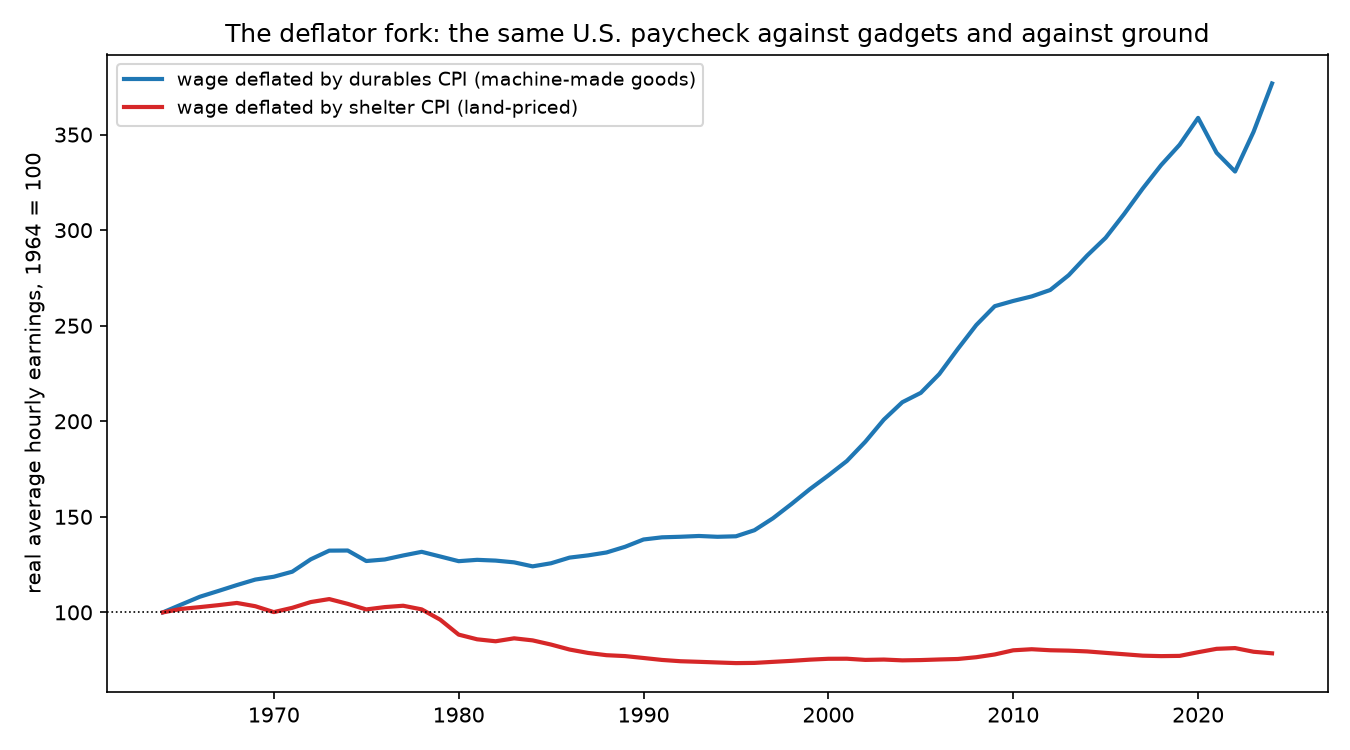
\includegraphics[width=0.88\linewidth]{figures/fig_deflator_fork.png}
\caption{The real-wage fork: U.S. average hourly earnings (production and nonsupervisory) deflated by the durables CPI and by the shelter CPI, 1964 = 100, complete calendar years through 2024. The fork ratio reaches $4.8\times$.}
\label{fig:fork}
\end{figure}

\textbf{The floor's coverage.} If the state captured every dollar of site rent and mailed each person an equal check, what fraction of one person's subsistence would it buy? Appendix~\ref{app:coverage} derives this coverage ratio $\kappa$ inside the model; Figure~\ref{fig:kappa} measures it: aggregate site-rent flow (land residuals from the Federal Reserve's Z.1 accounts --- market value minus replacement-cost structures --- under capitalization-rate variants, with the housing-services flow as a lower-bound member) against population times a costed subsistence bundle. $\kappa = 0.33$ [0.18--0.59] in 2025, up from roughly 0.05 in the 1950s --- the same $q$ that erodes the wage and the exit value has been raising the replacement base for seventy years, as Proposition~\ref{prop:fork}(ii) says it should. Two caveats. Every land measure used is a lower bound, so the truth likely sits above the band's middle. And $\kappa$'s upper bound is physical: coverage can never exceed the land-per-head ratio.

\begin{figure}[t!]
\centering
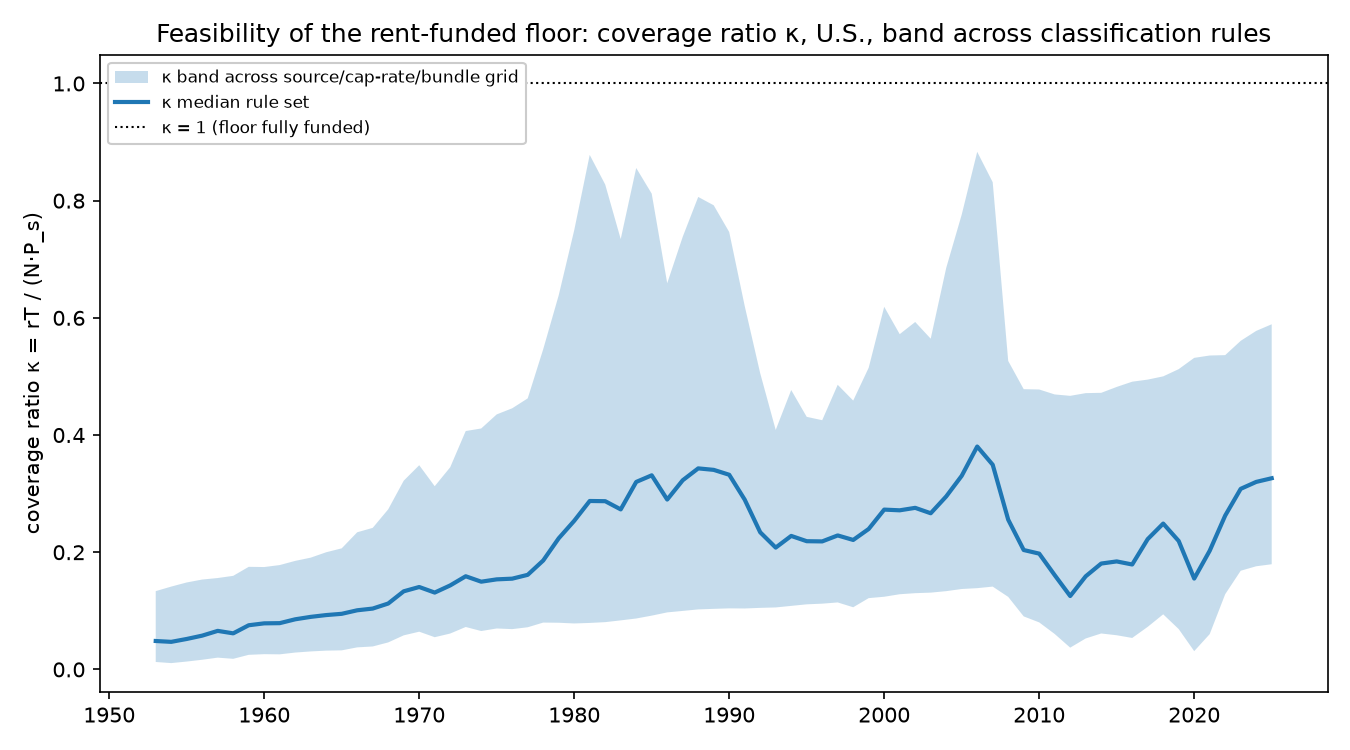
\includegraphics[width=0.88\linewidth]{figures/fig_kappa.png}
\caption{Coverage ratio $\kappa = rT/(N\cdot P_s)$ --- site rents $rT$ against population $N$ times the subsistence bundle's cost $P_s$ --- U.S., 1953--2025: median and min--max band across the land-source $\times$ capitalization-rate $\times$ bundle grid. Band width is substantially the capitalization-rate spread; the Z.1-residual members measure land as market value minus estimated structure replacement cost, an estimate known to be unreliable after 1995, and their business-structure coverage ends in 2020.}
\label{fig:kappa}
\end{figure}

\textbf{The fiscal exposure.} On the same accounts, 0.72 [0.66--0.81] of U.S. consumption financing is wage-linked and 0.68 of tax revenue is wage-exposed (2025) --- the state taxes precisely the base the technology erodes; the full ledger is Appendix~\ref{app:fiscal}'s table and Figure~\ref{fig:fourway}.

\textbf{Three possible interpretations of existing measures} (1) \emph{The slope from incidence:} under Proposition~\ref{prop:margin}, worker-borne payroll-tax shares map to the inverse slope of the schedule at the margin; the quasi-experimental estimates --- ranging from effectively full shifting onto wages (Gruber 1997) through partial (Kugler and Kugler 2009: formal wages fall 1.4--2.3\% per 10\% payroll-tax rise) to limited short-run shifting with firm-side responses (Saez, Schoefer, and Seim 2019) --- assembled chronologically on a common pass-through definition, would read the schedule's flattening as a time series. (2) \emph{$\lambda$:} the labor content of machine production is an input-output object --- the labor share of the machine-producing and machine-operating sectors, and the resolution of a unit of machine-intensive output into wages versus terminal rents after recursively removing intermediates, the empirical counterpart of the matrix recursion $\mathbf{c} = \mathbf{A}\mathbf{c} + \boldsymbol{\Lambda}w + \mathbf{B}\mathbf{r}$ of Appendix~\ref{app:environment}. Recursive automation appears as this series falling. (3) \emph{The long record:} welfare ratios (Allen 2001; Clark 2005) against long-run land-share series, spanning the two regime changes of Section~\ref{sec:history}, testing the joint reading flagged there.

\textbf{The rival for the shelter leg.} Zoning and supply restriction are the standing explanation for expensive housing: an institutional restriction is a chosen scarcity, and loosening it would move $q$. Two replies to that explanation. The durables leg of the fork owes nothing to housing policy, and its rise is the larger share of the divergence. And the model's claim is about where value migrates \emph{given} whatever stocks are scarce --- chosen scarcity is still scarcity, and its rents still land where Section~\ref{sec:limit} says; what zoning changes is how much of the scarcity is elective, which matters enormously for policy and not at all for the accounting. The discriminating evidence is cross-sectional, the fork's slope against local regulation and local exposure.

\section{Possible stabilizers}\label{sec:stabilizers}

Three possible stabilizers are granted as preserving real wages if $\gamma$ tends to $\bar{\gamma}$, however none of them exist without deadweight. Human-essential tasks can persist by preference or by law --- Appendix~\ref{app:human} grants the mechanism its theorem and shows the rescue is distributionally hollow where it operates (aggregate labor share saved, median wage not). Institutions can reserve work for people outright; that is a real instrument, and it is quantity protection rather than price protection. And supply expansion --- building, densifying, powering --- directly loosens the terminal constraint; it is the one lever that attacks $q$ itself.

The wedge result behind that distinction is Acemoglu and Restrepo's (2026). Let a task pay a premium over the base wage --- a union premium, a licensing rent, an efficiency wage --- as a multiplicative wedge $\mu (x) > 1$. Labor then holds the task only while $w \le c\cdot \gamma (x)/\mu (x)$: allocation runs on the wedge-deflated schedule, a premium raises its own task's flip priority one-for-one, and automation is directed at the best-paid versions of each job --- their targeting result, with the documented losses concentrated in the 70th--95th within-group percentiles. Any protection that operates through the price of labor therefore finances its own replacement; protection survives only in quantity form --- a scope-of-practice rule extended to software, an enforceable automation ban, a mandated human in the loop. Under pressure, protection converts from price form toward legal form, and adoption at legally blocked tasks turns punctuated: nothing moves while the saving from flipping runs below the cost of confrontation; past it, everything the rule covers flips at once.

\section{Implications for artificial intelligence, and conclusion}\label{sec:ai}

AI is the first technology that very plausibly moves both automation margins at once. It lowers $\gamma ^*$ wherever models reach parity at final tasks --- and it lowers $\lambda$, because software generation, chip design, datacenter operation, logistics, and research are themselves the machine sector's labor. The strong scenario of this paper requires both empirically: capability closing faster than reinstatement replenishes it, and the machine-production network shedding its own labor. If neither happens, the flat limit is a curiosity. If both do, the direction of travel is the one derived here: the wage's ceiling and floor converge, and the released value settles as rents on sites, power, water, minerals, and whatever law elects to protect --- not on the reproducible capital, whose price the recursion competes away. The prediction for the AI buildout itself is specific: model weights are ideas, copiable and distillable (distillation: cheaply training one model to imitate another); the durable balance-sheet items are the datacenters, the land under them, the power contracts, and the water rights.

One timing fact changes the policy conclusion: the same relative price $q$ that lowers the wage and erodes the exit option also raises the value of the base that could replace both. Coverage of a rent-funded floor has climbed from 0.05 to one-third in seventy years because the same rising rent that opens the fork is the coverage ratio's numerator. Necessity and feasibility travel together on one parameter, while the fiscal system keys 0.68 of its revenue to the base that is thinning. The pair of Proposition~\ref{prop:welfare} is where that mismatch resolves: a tax whose base cannot contract, funding a transfer that moves no margin, delivering redistribution without deadweight exactly where every wage-keyed instrument goes degenerate. Whether the economy arrives at the limit is an empirical question that is hard to measure at the scale of every good and policy system, yet what to do if it does is not an open question, and the instruments are old. The transition mechanics --- which bases bridge the crossing, at what deadweight, on what timetable --- are priced in Appendix~\ref{app:fiscal} and developed in a sequel.

This gives us the final empirical question that likely must be answered soon: is the economy's price recursion becoming less wage-linked and more scarcity-linked, and is the same scarcity eroding the value of exit?

\appendix
\counterwithin{proposition}{section}
\titleformat{\section}{\normalfont\Large\bfseries}{Appendix~\thesection.}{0.6em}{}

\section{The environment and assignment equilibrium}\label{app:environment}

The economy below generalizes the model of Sections~\ref{sec:model}--\ref{sec:floor}; the main text is the case with every extension absent --- one machine type, no reserved tasks, no government --- and each appendix relaxes one restriction. Notation is defined here once, and the machine sector's general form --- many machine types, durability --- is stated here as well. Every result is proved in the configuration it states, with the remaining restrictions in place; existence for the unrestricted economy is not claimed.

\textbf{Tasks and technology.} A final good requires a continuum of tasks $x \in$ [0,1] in equal amounts (Section~\ref{sec:model}). One human-hour completes $\gamma _L(x)$ units of task $x$, one machine-hour $\gamma _M(x)$; relative human productivity is $\gamma (x) = \gamma _L(x)/\gamma _M(x)$. A set $H$ of measure $|H| \ge 0$ is closed to machines --- by capability, preference, or law (Appendix~\ref{app:human}).

\textbf{Machines.} Machine services are produced. With one machine type, a unit takes $a$ units of machine services, $\lambda$ labor-hours, and $b$ units of non-produced services renting at $r$ (Section~\ref{sec:ceiling}). With many produced inputs, $\mathbf{c}$ is the vector of their prices, $\mathbf{A}$ the produced-input requirements matrix, $\boldsymbol{\Lambda}$ the labor requirements, $\mathbf{B}$ the requirements of terminal inputs with rent vector $\mathbf{r}$; free entry gives $\mathbf{c} = \mathbf{A}\mathbf{c} + \boldsymbol{\Lambda}w + \mathbf{B}\mathbf{r}$, hence $\mathbf{c} = (I-\mathbf{A})^{-1}(\boldsymbol{\Lambda}w + \mathbf{B}\mathbf{r})$ provided the spectral radius of $\mathbf{A}$ is below one --- the many-good statement of net reproduction. The scalar text carries the full logic: produced-input prices pass backward until anchored by factors outside the recursion and, during transition, by the labor still embodied in produced inputs. The task margin selects which machine type is the binding alternative at $x^*$: the one minimizing delivered task cost, and the threshold condition holds against that minimum. Free entry prices every produced input at unit cost.

\textbf{Durability, time preference, horizon.} With one-period building and time preference $\rho$ (the interest rate, distinct from the rent $r$), the $\lambda = 0$ recursion becomes $c = br(1+\rho )/(1 - a(1+\rho ))$, finite iff $a(1+\rho ) < 1$; with wear at rate $\delta$, the user-cost recursion gives $c = br(\rho +\delta )/(1 - a(\rho +\delta ))$. With $\lambda > 0$ the same closures hold with the recipe's labor priced at the margin: $c = br(1+\rho )/(1 - (1+\rho )(a + \lambda \gamma ^*))$ and $c = br(\rho +\delta )/(1 - (\rho +\delta )(a + \lambda \gamma ^*))$, finite iff $(1+\rho )(a + \lambda \gamma ^*) < 1$, respectively $(\rho +\delta )(a + \lambda \gamma ^*) < 1$. The added term is interest --- the wage of waiting --- competitive and real; it extends the income taxonomy without changing any destination. (These displays are computer-algebra-checked.) Whether an input is terminal is horizon-relative: transformer capacity is terminal over five years and produced over twenty; land is terminal at every horizon. The propositions hold per horizon with the classification made explicit, and our permanent-case claims use land alone.

\textbf{Non-produced inputs.} Terminal stocks are fixed: $T_j$ at rent $r_j$ where several matter (Section~\ref{sec:fiscal}), land the permanent case --- parcels of heterogeneous quality, reservation rent zero at the idle margin, rent schedule $r$(z) over parcels z (Appendix~\ref{app:landonly}). Land serves machine production and households: housing, and the $h_e$ units an independent exit requires.

\textbf{People.} $N$ workers each supply one hour or exit; types may differ in schedules and outside options (heterogeneous workers, below). Exit yields the keep $s_0$ on $h_e$ units of land, degrading to the dependency floor $\underline{s}$: $s(q) = \max(s_0 - q\cdot h_e, \underline{s})$ (Section~\ref{sec:floor}). Households spend on the machine-made good and direct land services, CES with weight $\alpha$ and elasticity $\sigma$; $\sigma = 1$ is Appendix~\ref{app:landonly}'s Cobb--Douglas, and general $\sigma$ is stated there.

\textbf{Government.} Four instruments: a payroll tax $\tau _w$ (Section~\ref{sec:fiscal}); a tax $\tau _R$ on pure ownership rents of terminal factors, returned as the uniform per-person transfer $d = \tau _R R/N$ (Section~\ref{sec:fiscal}); a uniform consumption tax (\ref{app:mix}); and a transfer program --- the pair $(m_w, m_e)$, what it pays per period in work and out of it (\ref{app:conditionality}).

\textbf{Equilibrium.} An equilibrium of a configuration is prices ($w, c, r$(z)), a task assignment, and a participation set such that every task is held by the input that costs less at ruling prices, free entry holds in machine production, the land market clears, and each worker participates exactly when work beats exit at the ruling prices and transfers. The configurations:

\begin{center}
{\small
\begin{tabular}{l p{8.6cm}}
\toprule
Where & Configuration \\
\midrule
Main text, Sections~\ref{sec:model}--\ref{sec:limit} & one machine type, $H = \emptyset$, no government \\
Section~\ref{sec:fiscal} & the rent tax and dividend $(\tau _R, d)$; the payroll contrast $\tau _w$ \\
Appendix~\ref{app:landonly} & the limit: $\gamma$ flat, $\lambda = 0, \rho = 0$; $\sigma = 1$, then general $\sigma$ \\
Appendix~\ref{app:fiscal} & government in full, sloped regime \\
Appendix~\ref{app:human} & $H$ of positive measure; $\gamma \to 0$ outside $H$ \\
\bottomrule
\end{tabular}
}
\end{center}

\begin{lemma}[existence and uniqueness]\label{lem:existence}
With the relabeled $\gamma$ continuous and strictly increasing where labor is employed, an equilibrium pair $(w, x^*)$ exists and is unique for any participant count; on a flat stretch the wage is pinned and only the assignment of identical-cost tasks is indeterminate, with nothing riding on it.
\end{lemma}

\begin{proof}
Absorbing more participants requires labor to hold more tasks, so the market-clearing wage $c\cdot \gamma (x^*(N_a))$, with $N_a$ the participant count, is continuous and strictly decreasing in $N_a$; participation supply is a step at $s$. A strictly decreasing continuous curve crosses a step exactly once, with Proposition~\ref{prop:margin}(iii) resolving the below-$s$ branch; flat stretches pin the wage at $c\cdot \bar{\gamma}$ and leave free only a measure-preserving relabeling.
\end{proof}

\textbf{The joint system.} With the recursion active, $c$ depends on $x^*$ through the machine sector's wage bill: $c(x^*) = br/(1 - a - \lambda \gamma (x^*))$ given $r$, and $w(x^*) = \gamma (x^*)\cdot c(x^*)$. Both are increasing in $\gamma (x^*)$ on the viable set $(\partial w/\partial \gamma ^* = br(1-a)/(1-a-\lambda \gamma ^*)^2 > 0)$, so the market-clearing wage remains strictly decreasing in the participant count and Lemma~\ref{lem:existence}'s crossing argument survives unchanged. Full equilibrium adds two more prices: $r$ clears the fixed land stock against machine-sector demand ($b$ per unit of gross machine services) plus housing demand, and $s = s(q)$ from Proposition~\ref{prop:exit}. Monotonicity is preserved at each layer --- more participants lower $w$, lower machine costs, raise land demand. Existence is claimed at three scopes, each with its own instrument: at given $r$, the crossing argument above; in the flat limit, the closed form of Appendix~\ref{app:landonly}, where clearing is solved exactly; and for the joint sloped system with $r$ endogenous, a numerical instantiation --- the check files solve a worked configuration for $(w, c, r, x^*)$ with land and labor clearing simultaneously and exhibit a unique crossing. A general fixed-point proof for the joint system is not claimed. Labor-market clearing counts both employments: final tasks plus $\lambda$ hours per unit of gross machine services.

\textbf{Heterogeneous workers.} With type-specific schedules and outside options, every proposition applies type by type; the aggregate schedule is the upper envelope of type schedules and the participation step becomes a distribution of steps. Floor statements refer to the bottom of the support.

\section{The land-only closure}\label{app:landonly}

Take Appendix~\ref{app:environment}'s economy to the full limit: $\gamma$ flat at $\bar{\gamma}, \lambda = 0, \rho = 0$, one terminal factor (land, homogeneous here; the heterogeneous case below), preferences at $\sigma = 1$ --- Cobb--Douglas with share $\alpha$ --- the stock $T$ jointly held and split between production use $T_P$ and housing $T_H$.

\begin{proposition}[closure and conservation of rents]\label{prop:landonly}
(i) Equilibrium exists with unique real allocation: $T_H = \alpha T, T_P = (1-\alpha )T$, final-good output $Y = (1-a)(1-\alpha )T/(b\bar{\gamma}\bar{L})$. (ii) The entire goods bill is production-land rent and national income is aggregate site rent identically: $pY = rT_P, pY + rT_H = rT$. (iii) Market clearing reproduces the cost-side relative price $r/p = (1-a)/(b\bar{\gamma}\bar{L})$: demand side and cost side agree on the same number.
\end{proposition}

\begin{proof}
Gross machine services solve $X = \bar{\gamma}\bar{L}Y + aX$, so $X = \bar{\gamma}\bar{L}Y/(1-a)$ and production land demand is $bX$. Substituting $p = br\bar{\gamma}\bar{L}/(1-a)$ gives $pY = r bX = rT_P$: goods spending passes through the zero-profit machine sector and accrues, all of it, to production land. Land being the only primary factor, household income is $rT$; Cobb--Douglas shares give $rT_H = \alpha rT$ and $pY = (1-\alpha )rT$; clearing pins $Y$ and dividing returns (iii).
\end{proof}

Dissipation is migration, by construction: the obvious escape --- automation's value dissipating into consumer surplus at collapsing prices --- is blocked, because prices do collapse \emph{and} the identity holds; what collapses is $p$ relative to $r$, never rent's claim on the flow of spending. \textbf{Heterogeneous parcels:} with a rent schedule over parcels in use and reservation rent zero at the idle margin, $rT$ reads $\int r$(z)$dz$ over parcels and nothing changes: the proposition requires only that spending, wherever it goes, crosses a site. \textbf{Labor still present at parity:} the identity weakens to ``all non-wage income is site rent,'' GDP $= N\cdot c\bar{\gamma} + rT$, recovering the full identity as $\bar{\gamma} \to 0$. \textbf{Feedback:} a rent-funded floor is spent partly on land services, lifting $r$ and the base $rT$ --- favorable in direction, distribution-dependent in size; claimed as tendency only.

\textbf{General $\bm{\sigma}$.} With the general elasticity $\sigma$ of Appendix~\ref{app:environment}'s preferences between goods and land services, the land share of expenditure becomes
\begin{equation}\label{eq:ces-share}
\alpha (q) = \alpha q^{1-\sigma} / (\alpha q^{1-\sigma} + 1 - \alpha ),
\end{equation}
and as automation sends $q$ up (Proposition~\ref{prop:fork}(ii)): $\alpha (q) \to 1$ for $\sigma < 1$ --- complements; housing takes the whole budget and the fork binds --- while $\alpha (q) \to 0$ for $\sigma > 1$ and substitution defuses it. The climbing shelter share of low-income budgets is the $\sigma < 1$ signature.

\section{The fiscal system in the sloped regime}\label{app:fiscal}

The main text proves what survives the limit; this appendix carries the transition results, plus the measured ledger --- Appendix~\ref{app:environment}'s government in full, in the sloped regime. Everything below passed the same check discipline as the main text.

\subsection{Conditionality}\label{app:conditionality}

A transfer program is Appendix~\ref{app:environment}'s pair $(m_w, m_e)$: what it pays per period in work and out of it. The worker compares $w + m_w$ against $s + m_e$, so the margin sees only $\Delta = m_w - m_e$ and the reservation wage is $s - \Delta$ (cash in exit also lifts the exit value itself --- an income effect the evidence puts small; Hoynes and Rothstein 2019). An in-work benefit $(\Delta > 0)$ recruits participation: in the sloped regime part of the benefit leaks into lower wages through the margin --- the Speenhamland result --- the 1795 poor-relief wage subsidies read as depressing wages --- rebuilt without employer power --- and at machine parity it induces work whose replacement value is below the outside option: society loses $s - c\bar{\gamma}$ per hour of employment so preserved. An out-of-work benefit $(\Delta < 0)$ raises the reservation wage and taxes the first hour; as parity compresses the wage distribution toward the floor, the mass of workers inside any fixed benefit-withdrawal (phase-out) band rises mechanically --- the trap worsens with no rule change. The uniform transfer is the unique $\Delta = 0$ instrument: zero compensated participation response as an identity. The three failure modes are one result read at three values of $\Delta$.

\subsection{Funding, and the incidence dial}\label{app:funding}

At the limit, a payroll-funded transfer is the closed loop of Section~\ref{sec:fiscal}; away from it, with labor-demand elasticity $\varepsilon _D$ (mapped by Proposition~\ref{prop:margin}(ii) to the inverse slope at the margin) and participation elasticity $\varepsilon _S$, workers bear $\varepsilon _D/(\varepsilon _D+\varepsilon _S)$ of a payroll tax, and exactly that fraction of a wage-funded transfer is circular: taken from the net wage, handed back as the transfer. The regime is therefore measurable: every payroll-incidence estimate is a reading of the schedule's slope, which is Section~\ref{sec:measurement}'s assembly (1). The land tax's properties (base cannot contract; capitalizes into price, not flow) hold at every point of the transition, not only at the limit --- which is why the pair of Proposition~\ref{prop:welfare} is close to a no-regret instrument: its non-distortion never depended on the limit arriving.

\subsection{Feasibility: the coverage ratio}\label{app:coverage}

Per person, subsistence is a bundle $(g_s, h_s)$ of goods and land services costing $P_s = p g_s + r\cdot h_s$; full capture of site rent funds $rT/N$ per head; coverage at full capture is $\kappa = rT/(N\cdot P_s) = qT/(N(g_s + q\cdot h_s))$, strictly increasing in $q$ toward the physical ceiling $T/(N\cdot h_s)$, with $\kappa \ge 1$ iff $q \ge q^* = N\cdot g_s/(T - N\cdot h_s)$ --- a finite threshold that exists iff $T > N\cdot h_s$. The fiscal constraint is a land constraint in disguise: the floor is fundable exactly when the direct plus embodied land content of $N$ bundles fits in the land there is. Measured: Section~\ref{sec:measurement}'s Figure~\ref{fig:kappa} (0.05 $\to 0.33$ [0.18--0.59], 1953--2025), with the ceiling caveat stated there. Worked instance ($a = 0.6, b = 0.2, \bar{\gamma} = 1.8, \bar{L} = 1$, so $q = 10/9$; $T = 100$; unit bundle): fifty people are covered with room to spare $(\kappa = 20/19)$; eighty must wait for $q$ to reach 4; one hundred twenty are never covered.

\subsection{The race with enclosure}\label{app:race}

Proposition~\ref{prop:exit}'s independent exit ends where rising rents exhaust the keep, at $q_{\mathrm{enc}} = (s_0-\underline{s})/h_e$; the fundable floor arrives at $q^*$. The natural floor outlasts the replacement's arrival iff $q_{\mathrm{enc}} \ge q^*$, i.e. iff $N \le q_{\mathrm{enc}}T/(g_s + q_{\mathrm{enc}}h_s)$ --- a crowding condition (60 people in the worked instance, where $q_{\mathrm{enc}} = 1.5$). Otherwise a gap opens --- commons gone, floor not yet fundable --- and transition instruments are rescue, not optimization. Two closing observations: the uniform transfer's cancellation survives any $s(q)$, and past $q_{\mathrm{enc}}$ the guaranteed floor is $\underline{s} + d$ --- the transfer replaces the commons rather than supplementing it, billed at exactly the $h_e\cdot q_{\mathrm{enc}}$ the enclosure took, funded from inside the $rT$ the enclosure created.

\subsection{The mix on the way down}\label{app:mix}

Until $\kappa$ reaches one, a full floor needs revenue beyond site rents, and the two reaching instruments miss opposite bases: a land tax reaches every site rent, saved or consumed, but no bottleneck profit or royalty; a uniform consumption tax reaches whatever finances consumption --- including exactly those non-site rents --- but its wage-financed slice is a payroll tax in disguise. With $\varphi _C$ the wage-financed share of consumption ($\varphi _G$, in the table, its tax-revenue counterpart), filling the rent base first is optimal (its marginal deadweight is zero at every rate), the consumption tax covers the shortfall, and minimized deadweight is proportional to $\varphi _C(1-\kappa )^2$ --- the product of two measured series, 0.72 and 0.33 today, giving 0.32; at (0.50, 0.60) it would be 0.08. Both series are moving the right way, the consumption tax is scaffolding by construction, and in the corollary's limit the bases merge (all consumption resolves into rent income by \ref{prop:landonly}) and the mix question disappears.

\begin{center}
{\small
\begin{tabular}{p{6.4cm} l p{4.6cm}}
\toprule
Object & Value (year) & Note \\
\midrule
Wage-linked share of consumption financing, $\varphi _C$ & 0.72 [0.66--0.81] (2025) & down from $\approx 0.80$ in 1965 \\
Wage-linked share of tax revenue, $\varphi _G$ & 0.68 (2025) & 0.64 in 1965; $\approx 0.70$ by the mid-1980s, flat since \\
Work- or means-conditioned share of benefits & $\ge 0.84$; $\approx 0.99$ by withdrawal rule (2024) & the only sizable unconditional cash transfer is Alaska's dividend \\
Coverage ratio $\kappa$ (\ref{app:coverage}) & 0.33 [0.18--0.59] (2025) & $\approx 0.05$ in the 1950s; land measures are lower bounds \\
Transition deadweight index $\varphi _C(1-\kappa )^2$ & 0.32 (2025) & both factors improving \\
\bottomrule
\end{tabular}
}
\end{center}

\begin{figure}[t!]
\centering
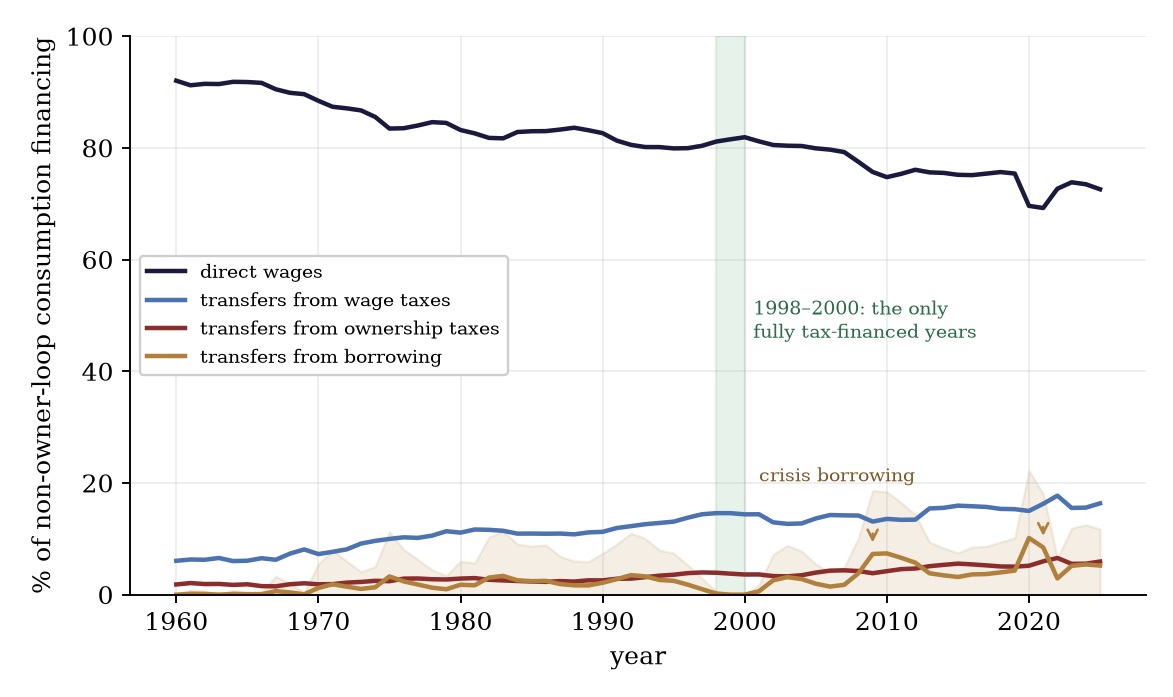
\includegraphics[width=0.88\linewidth]{figures/fig_fourway.png}
\caption{Financing of U.S. consumption outside the owner loop --- the slice financed directly by household capital income, owners consuming their own returns --- 1962--2025 (medians across the classification-rule grid; the shaded band spans deficit-attribution rules). Direct wages' share has ceded twenty points in sixty years in a ratchet: each recession lowers it, and each recovery restores only part. Transfers grew on a funding mix that stayed roughly quarter-ownership; the borrowed channel reached 19\% of transfers by 2025, and only in 1998--2000 did it vanish. Funding attribution is pro-rata accounting, not estimated incidence.}
\label{fig:fourway}
\end{figure}

\section{Human-essential tasks}\label{app:human}

Let Appendix~\ref{app:environment}'s set $H$ have positive measure $|H|$: tasks machines cannot hold --- by capability residue, by verified preference for human hands, or by law --- with $H$-wage $w_H$. Let machines grow unboundedly better at every task outside $H$: $\gamma (x) \to 0$ there, the stricter limit of Section~\ref{sec:limit}'s corollary confined to the tasks machines can hold. The machine rental $c$ stays pinned by the recursion; what vanishes is the per-task cost of machine work, $c/\gamma _M(x) = c\cdot \gamma (x)/\gamma _L(x)$. Aghion, Jones, and Jones (2019) raise the strongest stabilizer this paper faces: Baumol concentration --- expenditure concentrating on the sector whose costs refuse to fall (Baumol 1967), here the human-essential set --- can preserve labor's share indefinitely. Proposition~\ref{prop:baumol} grants the mechanism its theorem and makes its premise explicit.

\begin{proposition}[Baumol concentration]\label{prop:baumol}
(i) Any good whose task list contains $H$ has unit cost tending to $|H|\cdot w_H/\gamma _L$ as $\gamma \to 0$ outside $H$: labor's share of its cost tends to one. (ii) Under CES substitution $\sigma _H$ between $H$-content and $H$-light substitutes, the expenditure share of $H$-content tends to 1 if $\sigma _H < 1$, to the taste weight if $\sigma _H = 1$, and to 0 if $\sigma _H > 1$. (iii) On the $\sigma _H < 1$ branch with three categories (machine-made goods, land services, $H$-labor), end-state expenditure splits between the two non-collapsing categories --- land services and $H$-labor --- and labor's aggregate share tends to the $H$-share of that split. Our baseline is exactly the $H = \emptyset$ edge of this result.
\end{proposition}

\begin{proof}
(i) $H$-tasks cost $|H|\cdot w_H/\gamma _L$ whatever machines do; each task outside $H$ costs $c\cdot \gamma (x)/\gamma _L(x)$, and the recursion keeps $c$ bounded as $\gamma$ falls (Proposition~\ref{prop:replacement}), so the remainder vanishes with $\gamma$. (ii) is Appendix~\ref{app:landonly}'s share display with $q$ read as the relative price of $H$-content: the costlier category's share rises with its relative price iff $\sigma _H < 1$, and by (i) that relative price diverges. (iii) A $H$-free good's price vanishes by (i) at $|H| = 0$, so for $\sigma _H < 1$ its share vanishes, leaving the displayed split; setting the $H$ taste weight to zero returns the baseline.
\end{proof}

Two anchors, and a hollowness result. \emph{Credence (the buyer cannot verify provenance):} preference-based membership binds only if provenance can be verified: suppose buyers carry a taste premium for verified human work, verification catches a false claim with probability $v$, and a caught claim pays a penalty $f$.

\begin{lemma}[the fraud bound]\label{lem:fraud}
A premium on verified human work is sustainable only up to $v\cdot f/(1-v)$: at any higher premium, false claiming is profitable in expectation and entry by fakes competes the premium away. The bound rises in $v$ and in $f$, diverges as $v \to 1$, and collapses to zero as $f \to 0$ for every $v < 1$.
\end{lemma}

\begin{proof}
A false claimant earns the premium with probability $1 - v$ and pays $f$ with probability $v$; expected profit is nonpositive iff the premium is at most $v\cdot f/(1-v)$. The comparative statics and limits are elementary.
\end{proof}

With price-only enforcement $(f \to 0)$ the bound collapses for every $v < 1$: certified-human markets unravel through fakes, not robots. $H$'s durable core is what law reserves plus what co-presence verifies --- being in the room, where faking is impossible rather than merely punished. \emph{Superstars:} within $H$, the broadcastable fraction $\psi$ of demand concentrates on top performers (Rosen 1981) while only the co-present remainder is rationed by human capacity.

\begin{lemma}[superstar concentration]\label{lem:superstar}
Let the broadcastable fraction $\psi$ of $H$-expenditure accrue to a set of performers of measure zero, and let the co-present remainder be shared uniformly across the $H$-workforce. The mean $H$-income is unchanged, and the median $H$-income is $(1-\psi )$ times the mean.
\end{lemma}

\begin{proof}
Total $H$-income equals $H$-expenditure whatever its division; the stars carry the fraction $\psi$ on measure zero, every other worker receives the uniform share $(1-\psi )$ times the mean, and a measure-zero top moves no quantile below the top.
\end{proof}

Wherever $H$ employs a minority the economy-wide median worker holds no $H$-task at all, and on the $\sigma _H < 1$ branch the aggregate labor share can persist, even approach one, while the median wage collapses to the floor: aggregate rescue, median collapse. The Baumol case also raises the floor's price: care and teaching put human hours in the subsistence bundle. Extend \ref{app:coverage}'s bundle with $n_s$ hours of $H$-service and coverage becomes $\kappa = qT/(N\cdot (g_s + n_s\cdot w_H/p + q\cdot h_s))$ --- below the $H$-free ratio at every $q$, and further below as the $H$-hour's price rises.

\section*{References}

{\small\singlespacing
\refentry{Acemoglu, D., and D. Autor (2011). ``Skills, Tasks and Technologies: Implications for Employment and Earnings.'' In \emph{Handbook of Labor Economics}, vol. 4B. Elsevier.}
\refentry{Acemoglu, D., and P. Restrepo (2018). ``The Race between Man and Machine: Implications of Technology for Growth, Factor Shares, and Employment.'' \emph{American Economic Review} 108(6): 1488--1542.}
\refentry{Acemoglu, D., and P. Restrepo (2022). ``Tasks, Automation, and the Rise in U.S. Wage Inequality.'' \emph{Econometrica} 90(5).}
\refentry{Acemoglu, D., and P. Restrepo (2026). ``Automation and Rent Dissipation: Implications for Wages, Inequality, and Productivity.'' \emph{The Quarterly Journal of Economics} 141(2): 1521--1579.}
\refentry{Aghion, P., B. F. Jones, and C. I. Jones (2019). ``Artificial Intelligence and Economic Growth.'' In A. Agrawal, J. Gans, and A. Goldfarb (eds.), \emph{The Economics of Artificial Intelligence}, University of Chicago Press.}
\refentry{Allen, R. C. (2001). ``The Great Divergence in European Wages and Prices from the Middle Ages to the First World War.'' \emph{Explorations in Economic History} 38(4): 411--447.}
\refentry{Arnott, R. J., and J. E. Stiglitz (1979). ``Aggregate Land Rents, Expenditure on Public Goods, and Optimal City Size.'' \emph{The Quarterly Journal of Economics} 93(4): 471--500.}
\refentry{Arrow, K. J. (1951). ``An Extension of the Basic Theorems of Classical Welfare Economics.'' In \emph{Proceedings of the Second Berkeley Symposium on Mathematical Statistics and Probability}, University of California Press.}
\refentry{Autor, D. (2015). ``Why Are There Still So Many Jobs? The History and Future of Workplace Automation.'' \emph{Journal of Economic Perspectives} 29(3).}
\refentry{Autor, D., and D. Dorn (2013). ``The Growth of Low-Skill Service Jobs and the Polarization of the US Labor Market.'' \emph{American Economic Review} 103(5): 1553--1597.}
\refentry{Autor, D., F. Levy, and R. J. Murnane (2003). ``The Skill Content of Recent Technological Change: An Empirical Exploration.'' \emph{The Quarterly Journal of Economics} 118(4): 1279--1333.}
\refentry{Baumol, W. J. (1967). ``Macroeconomics of Unbalanced Growth: The Anatomy of Urban Crisis.'' \emph{American Economic Review} 57(3): 415--426.}
\refentry{Bouscasse, P., E. Nakamura, and J. Steinsson (2025). ``When Did Growth Begin? New Estimates of Productivity Growth in England from 1250 to 1870.'' \emph{The Quarterly Journal of Economics} 140(2): 835--888.}
\refentry{Card, D., A. R. Cardoso, J. Heining, and P. Kline (2018). ``Firms and Labor Market Inequality: Evidence and Some Theory.'' \emph{Journal of Labor Economics} 36(S1).}
\refentry{Caselli, F., and A. Manning (2019). ``Robot Arithmetic: New Technology and Wages.'' \emph{American Economic Review: Insights} 1(1).}
\refentry{Clark, G. (2005). ``The Condition of the Working Class in England, 1209--2004.'' \emph{Journal of Political Economy} 113(6): 1307--1340.}
\refentry{Crafts, N. (2022). ``Slow Real Wage Growth during the Industrial Revolution: Productivity Paradox or Pro-Rich Growth?'' \emph{Oxford Economic Papers} 74(1): 1--13.}
\refentry{Diamond, P. A. (1982). ``Aggregate Demand Management in Search Equilibrium.'' \emph{Journal of Political Economy} 90(5).}
\refentry{Diamond, P., and J. Mirrlees (1971). ``Optimal Taxation and Public Production I: Production Efficiency.'' \emph{American Economic Review} 61(1).}
\refentry{George, H. (1879). \emph{Progress and Poverty.}}
\refentry{Grossman, G. M., and E. Rossi-Hansberg (2008). ``Trading Tasks: A Simple Theory of Offshoring.'' \emph{American Economic Review} 98(5).}
\refentry{Gruber, J. (1997). ``The Incidence of Payroll Taxation: Evidence from Chile.'' \emph{Journal of Labor Economics} 15(3, Part 2): S72--S101.}
\refentry{Hagedorn, M., and I. Manovskii (2008). ``The Cyclical Behavior of Equilibrium Unemployment and Vacancies Revisited.'' \emph{American Economic Review} 98(4): 1692--1706.}
\refentry{Hall, R. E. (2005). ``Employment Fluctuations with Equilibrium Wage Stickiness.'' \emph{American Economic Review} 95(1).}
\refentry{Hémous, D., and M. Olsen (2022). ``The Rise of the Machines: Automation, Horizontal Innovation, and Income Inequality.'' \emph{American Economic Journal: Macroeconomics} 14(1).}
\refentry{Hoynes, H., and J. Rothstein (2019). ``Universal Basic Income in the United States and Advanced Countries.'' \emph{Annual Review of Economics} 11.}
\refentry{Jones, D., and I. Marinescu (2022). ``The Labor Market Impacts of Universal and Permanent Cash Transfers: Evidence from the Alaska Permanent Fund.'' \emph{American Economic Journal: Economic Policy} 14(2): 315--340.}
\refentry{Karabarbounis, L., and B. Neiman (2014). ``The Global Decline of the Labor Share.'' \emph{The Quarterly Journal of Economics} 129(1).}
\refentry{Knoll, K., M. Schularick, and T. Steger (2017). ``No Price Like Home: Global House Prices, 1870--2012.'' \emph{American Economic Review} 107(2).}
\refentry{Korinek, A., and J. E. Stiglitz (2019). ``Artificial Intelligence and Its Implications for Income Distribution and Unemployment.'' In A. Agrawal, J. Gans, and A. Goldfarb (eds.), \emph{The Economics of Artificial Intelligence}, University of Chicago Press.}
\refentry{Korinek, A., and D. Suh (2024). ``Scenarios for the Transition to AGI.'' NBER Working Paper 32255.}
\refentry{Kugler, A., and M. Kugler (2009). ``Labor Market Effects of Payroll Taxes in Developing Countries: Evidence from Colombia.'' \emph{Economic Development and Cultural Change} 57(2): 335--358.}
\refentry{Leontief, W. W. (1936). ``Quantitative Input and Output Relations in the Economic Systems of the United States.'' \emph{The Review of Economics and Statistics} 18(3): 105--125.}
\refentry{Lewis, W. A. (1954). ``Economic Development with Unlimited Supplies of Labour.'' \emph{The Manchester School} 22(2): 139--191.}
\refentry{Ljungqvist, L., and T. J. Sargent (2017). ``The Fundamental Surplus.'' \emph{American Economic Review} 107(9): 2630--2665.}
\refentry{Malthus, T. R. (1798). \emph{An Essay on the Principle of Population.}}
\refentry{Manning, A. (2003). \emph{Monopsony in Motion: Imperfect Competition in Labor Markets.} Princeton University Press.}
\refentry{Mas, A., and A. Pallais (2019). ``Labor Supply and the Value of Non-Work Time: Experimental Estimates from the Field.'' \emph{American Economic Review: Insights} 1(1): 111--126.}
\refentry{Moll, B., L. Rachel, and P. Restrepo (2022). ``Uneven Growth: Automation's Impact on Income and Wealth Inequality.'' \emph{Econometrica} 90(6).}
\refentry{Mortensen, D. T., and C. A. Pissarides (1994). ``Job Creation and Job Destruction in the Theory of Unemployment.'' \emph{The Review of Economic Studies} 61(3): 397--415.}
\refentry{Piketty, T., and G. Zucman (2014). ``Capital is Back: Wealth-Income Ratios in Rich Countries 1700--2010.'' \emph{The Quarterly Journal of Economics} 129(3).}
\refentry{Pissarides, C. A. (2000). \emph{Equilibrium Unemployment Theory.} 2nd ed., MIT Press.}
\refentry{Polanyi, K. (1944). \emph{The Great Transformation.}}
\refentry{Ricardo, D. (1817). \emph{On the Principles of Political Economy and Taxation.} Third edition, 1821, adds the chapter ``On Machinery.''}
\refentry{Rognlie, M. (2015). ``Deciphering the Fall and Rise in the Net Capital Share.'' \emph{Brookings Papers on Economic Activity.}}
\refentry{Romer, P. M. (1990). ``Endogenous Technological Change.'' \emph{Journal of Political Economy} 98(5): S71--S102.}
\refentry{Rosen, S. (1981). ``The Economics of Superstars.'' \emph{American Economic Review} 71(5).}
\refentry{Sachs, J. D., and L. J. Kotlikoff (2012). ``Smart Machines and Long-Term Misery.'' NBER Working Paper 18629.}
\refentry{Saez, E., B. Schoefer, and D. Seim (2019). ``Payroll Taxes, Firm Behavior, and Rent Sharing: Evidence from a Young Workers' Tax Cut in Sweden.'' \emph{American Economic Review} 109(5): 1717--1763.}
\refentry{Samuelson, P. A. (1966). ``A Summing Up.'' \emph{The Quarterly Journal of Economics} 80(4).}
\refentry{Shapiro, C., and J. E. Stiglitz (1984). ``Equilibrium Unemployment as a Worker Discipline Device.'' \emph{American Economic Review} 74(3): 433--444.}
\refentry{Shimer, R. (2005). ``The Cyclical Behavior of Equilibrium Unemployment and Vacancies.'' \emph{American Economic Review} 95(1): 25--49.}
\refentry{Sraffa, P. (1960). \emph{Production of Commodities by Means of Commodities.} Cambridge University Press.}
\refentry{Susskind, D. (2017). ``A Model of Technological Unemployment.'' Oxford Department of Economics Discussion Paper 819.}
\refentry{Uzawa, H. (1961). ``Neutral Inventions and the Stability of Growth Equilibrium.'' \emph{The Review of Economic Studies} 28(2): 117--124.}
\refentry{Zeira, J. (1998). ``Workers, Machines, and Economic Growth.'' \emph{The Quarterly Journal of Economics} 113(4).}
}

\bigskip\par\noindent\rule{0.35\linewidth}{0.4pt}\par\smallskip
\noindent{\footnotesize\singlespacing \textbf{Data and computation.} All U.S. figures are gross annual flows computed from BEA national accounts (annual NIPA series retrieved via FRED, 2026 vintage), with Federal Reserve Z.1 balance-sheet lines, BEA fixed-assets stocks, and the CPI for the coverage ratio, and HUD FY2025 fair-market rents for the ceiling grid. Series windows follow their sources: financing splits 1962--2025, coverage ratio 1953--2025, deflator fork 1964--2024 on complete calendar years. Every arguable classification was computed under all defensible variants; reported values are medians with min--max bands across the rule grid. Flows are gross. \textbf{Notation.} The machine-recipe labor coefficient $\lambda$ is unrelated to the wage-linkage shares $\varphi _C, \varphi _G$ of Appendix~\ref{app:fiscal} and to Acemoglu--Restrepo's task-substitution elasticity $\lambda$; rent is $r$ (aggregate $R$) while the interest rate is $\rho$; the wedge $\mu$ appears only in Section~\ref{sec:stabilizers}; the CES elasticities are $\sigma$ (goods versus land services, Appendix~\ref{app:landonly}) and $\sigma _H (H$-content versus substitutes, Appendix~\ref{app:human}); the human-essential set $H$ is unrelated to the housing subscript of $T_H$; and the outside option $s$ is a price this paper constructs, not search theory's exogenous value of non-market activity, whose customary symbol $b$ is the land coefficient here.\par}

\bigskip\par\noindent\rule{0.35\linewidth}{0.4pt}\par\smallskip
\noindent{\footnotesize\singlespacing \textbf{Verification.} Every proposition's algebra is checked by computer algebra (sympy) and its equilibrium claims against numerical instantiations; the check files ship with the repository. The full-automation chain --- the $\lambda = 0$ recursion, the closure identity, the fork, the funding and conditionality results, and the welfare pair --- is also stated and proved in Lean 4 (with the mathlib library), as are the $\lambda > 0$ closure and its comparative statics (Propositions~\ref{prop:replacement} and \ref{prop:fork}(i)--(ii)), the user-cost closures, Lemmas \ref{lem:fraud} and \ref{lem:superstar}, and Appendix~\ref{app:landonly}'s CES share limits. The Lean development carries an assumption manifest --- the enumerated hypotheses each proposition consumes --- and its statements are a translation of the paper's: the proofs are machine-checked, the translation is not. The joint-system fixed point of Appendix~\ref{app:environment} is outside the formalization, as stated there.\par}

\bigskip\par\noindent\rule{0.35\linewidth}{0.4pt}\par\smallskip
\noindent{\footnotesize\singlespacing \textbf{AI use.} This paper was written in collaboration with Claude (Anthropic). The theory and its central claims are the author's; the formalization, proofs, computations, figures, and nearly all of the prose were drafted by Claude under the author's direction and review. All data were pulled live from public sources; the code and data are public. Errors remain the author's.\par}

\end{document}
